\chapter{A chapter}
\label{cha:a_chapter}

This is the first paragraph of the \PolyTeXnic\ template. It shows how to write a document in \PolyTeX, a subset of the \LaTeX\ typesetting language optimized for ebooks. For more information, see \emph{The \PolyTeXnic\ Book}, available online at \href{http://polytexnic.org/book}{http://polytexnic.org/book}, and the \PolyTeX\ source of the book, available at \href{http://polytexnic.org/source}{http://polytexnic.org/source}. To learn how to easily publish (and optionally sell) documents produced with \PolyTeXnic, visit \href{http://softcover.io/}{Softcover.io}.

This is the \emph{second} paragraph, showing how to emphasize text.\footnote{This is a footnote. It is numbered automatically.} You can also make text \textbf{bold} or \textit{italicized} (which looks the same as emphasized text).

\emph{Note}: ``\PolyTeXnic'' is pronounced exactly like the English word \emph{polytechnic}, and ``\LaTeX'' is pronounced \emph{lay}-tech (with ``tech'' as in ``technology'').\footnote{Pronunciations of ``\LaTeX'' differ, but \emph{lay}-tech is the one I prefer.}

\section{A section}
\label{sec:a_section}

This is a section. Because it has a label, we can refer to it as Section~\ref{sec:a_section}. The cross-reference will be automatically numbered and linked. There's another reference to this section in Section~\ref{sec:floats}, as well as one in Chapter~\ref{cha:another_chapter}.

\subsection{Source code}
\label{sec:source_code}

This is a subsection. As usual, it can be referenced by label (Section~\ref{sec:source_code}). Note that the label starts with \kode{sec:}, not \kode{ssec:} or \kode{subsec:}. Any of these would work, but I find that sections often become subsections (and vice versa) when figuring out the structure of a book, and using \kode{sec:} to prefix them both saves having to change labels.

\PolyTeXnic\ comes with full support for syntax-highlighted source code:
%= lang:ruby
\begin{code}
def hello
  puts "hello, world!"
end
\end{code}
\noindent \PolyTeXnic\ can highlight any language supported by \href{http://pygments.org/languages/}{Pygments} (which means most of them).

You can also define \emph{code listings}, as seen in Listing~\ref{code:hello_world}. Such code listings are automatically numbered and linked.

\begin{codelisting}
\label{code:hello_world}
\codecaption{``Hello, world!'' in Ruby.}
%= lang:ruby
\begin{code}
def hello
  puts "hello, world!"
end
\end{code}
\end{codelisting}

You can indicate inline code with the \verb+\kode+ command, as in \kode{current\_\-user}. If you prefer a plainer version of the same thing, you can use ``typewriter text'', as in \texttt{current\_\-user}.

For words whose hypenation isn't built in, you can indicate an optional hyphen using \verb+\-+ (Listing~\ref{code:hyphenation}), which will only be used if necessary to make a clean line break (and even then only when producing PDFs). You can also define global hyphenation rules in \texttt{custom.sty}, which includes a rule for hyphenating ``JavaScript''.

\begin{codelisting}
\label{code:hyphenation}
\codecaption{Adding an optional hyphen to \kode{current\_user}.}
%= lang:latex
\begin{code}
current\_\-user
\end{code}
\end{codelisting}

Listing~\ref{code:hyphenation} also shows how to escape the underscore character using a backslash. This is necessary because plain underscores are reserved for math environments (Section~\ref{sec:mathematics}).

\subsection{Mathematics}
\label{sec:mathematics}

\PolyTeXnic\ supports full mathematical typesetting, including inline math, such as $\phi^2 - \phi - 1 = 0$, and centered math, such as
\[ \phi = \frac{1+\sqrt{5}}{2}. \]
It also supports cross-referenced equations, as in Eq.~\eqref{eq:golden_ratio} and Eq.~\eqref{eq:stokes_theorem}. Math support for HTML, EPUB, and MOBI comes via the amazing \href{http://www.mathjax.org/}{MathJax} JavaScript library, which includes the American Mathematical Society extensions (AMS-\LaTeX) as well as all the default \LaTeX\ math commands.

\begin{equation}
\label{eq:golden_ratio}
\phi = \frac{1+\sqrt{5}}{2} \approx 1.618 \qquad{\text{The Golden Ratio}}
\end{equation}

\begin{equation}
\label{eq:stokes_theorem}
\int_\Omega d\omega = \int_{\partial\Omega} \omega \qquad{\text{Generalized Stokes's Theorem}}
\end{equation}

As with all \PolyTeXnic\ features, mathematical typesetting is fully supported in all output formats (HTML, EPUB, MOBI, and PDF). The only caveat is that, due to technical restrictions imposed by e-readers, math typesetting is not quite as pretty in EPUB \& MOBI. Future versions of \PolyTeXnic\ will include even nicer EPUB \& MOBI math typesetting as the capabilities of those formats improve.

\section{Floats}
\label{sec:floats}

This is the second section. As we saw above above, the first section is Section~\ref{sec:a_section}.

\PolyTeXnic\ supports \href{http://en.wikibooks.org/wiki/LaTeX/Floats,_Figures_and_Captions}{\emph{floats}} such as figures and tables, including numbered captions and linked cross-references. The defining quality of a float is that its placement isn't guaranteed (i.e., it ``floats'' in the document), so you shouldn't generally assume it will be placed immediately after the text that precedes it. (Such placement \emph{will} be the case with HTML-based output, but \emph{not} in PDFs, where \TeX's state-of-the-art float placement algorithm is in charge.)

\subsection{Graphics and figures}
\label{sec:graphics_and_figures}

You can include raw graphics like this:

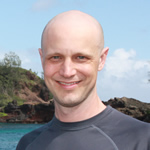
\includegraphics{images/2011_michael_hartl.png}

\noindent You can also include centered images like this:

\image{images/2011_michael_hartl.png}

\noindent Or put a box around it, like so:

\imagebox{images/2011_michael_hartl.png}

To turn it into a figure, use the \kode{figure} environment (Figure~\ref{fig:the_dude}).

\begin{figure}
\imagebox{images/2011_michael_hartl.png}
\caption{Some \href{http://michaelhartl.com/}{dude}.\label{fig:the_dude}}
\end{figure}

\subsection{Tables and tabular environments}
\label{tables_and_tabular}

\PolyTeXnic\ supports raw tables via the \kode{tabular} environment.

\begin{tabular}{llll}
\textbf{HTTP request} & \textbf{URL} & \textbf{Action} & \textbf{Purpose} \\ \hline

\texttt{GET} & /users & \texttt{index} & page to list all users \\
\texttt{GET} & /users/1 & \texttt{show} & page to show user with id \texttt{1}\\
\texttt{GET} & /users/new & \texttt{new} & page to make a new user \\
\texttt{POST} & /users & \texttt{create} & create a new user \\
\texttt{GET} & /users/1/edit & \texttt{edit} & page to edit user with id \texttt{1} \\
\texttt{PATCH} & /users/1 & \texttt{update} & update user with id \texttt{1}  \\
\texttt{DELETE} & /users/1 & \texttt{destroy} & delete user with id \texttt{1}
\end{tabular}

To make a tabular environment into a full-blown table, with a number and a caption, use the \kode{table} environment (Table~\ref{table:rails_actions}).

\begin{table}
\begin{tabular}{llll}
\textbf{HTTP request} & \textbf{URL} & \textbf{Action} & \textbf{Purpose} \\ \hline

\texttt{GET} & /users & \texttt{index} & page to list all users \\
\texttt{GET} & /users/1 & \texttt{show} & page to show user with id \texttt{1}\\
\texttt{GET} & /users/new & \texttt{new} & page to make a new user \\
\texttt{POST} & /users & \texttt{create} & create a new user \\
\texttt{GET} & /users/1/edit & \texttt{edit} & page to edit user with id \texttt{1} \\
\texttt{PATCH} & /users/1 & \texttt{update} & update user with id \texttt{1}  \\
\texttt{DELETE} & /users/1 & \texttt{destroy} & delete user with id \texttt{1}
\end{tabular}
\caption{The default \href{http://rubyonrails.org/}{Rails} actions.\label{table:rails_actions}}
\end{table}

\section{Miscellanea}

Apart from two mostly empty chapters (Chapter~\ref{cha:another_chapter} and Chapter~\ref{cha:yet_another_chapter}), this is the end of the template. In fact, let's include Chapter~\ref{cha:yet_another_chapter} in its entirety, just to see how mostly empty it is:

%= << chapters/yet_another_chapter.tex

To learn more about what \PolyTeXnic\ can do, visit \href{http://polytexnic.org/book}{http://polytexnic.org/book}.